% 2026-10-18 (step 2): rewritten against the CDC reviews and the code. Frame construction
% (R5 #1), position-only miss (R8 #2), evader/pursuer indices (R8 #3), both LPs in the
% correct sign convention (R7 #2-3, R8 #1), "game value" reserved for the LP value (R7 #6),
% beliefs FP-only with distinct symbols (R7 m2, R8 #4), greedy labelled a heuristic (R7 #4),
% FP-mixed defined (R7 #5), and the trajectory problem stated as actually solved (R7 #1).

To avoid the issues of equilibrium non-existence and deterministic strategies, we replace the continuous control space with a lifted game played over a finite set of candidate trajectories. Each game step, both players generate candidates, the resulting matrix game is solved for a mixed equilibrium, and each player selects a candidate according to its strategy, which may use beliefs about the opponent learned online.

\begin{figure*}[!t]
    \centering
    \begin{subfigure}{0.32\linewidth}
        \centering
        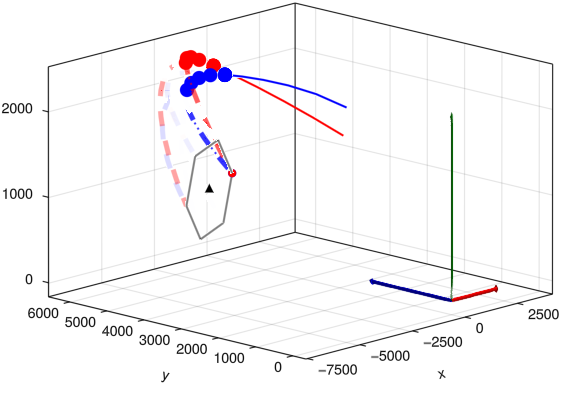
\includegraphics[width=\linewidth]{images/k_replan_1.png}
        \caption{Game step $s = 2$ }
        \label{fig:k_replan_1}
    \end{subfigure}
    \begin{subfigure}{0.32\linewidth}
        \centering
        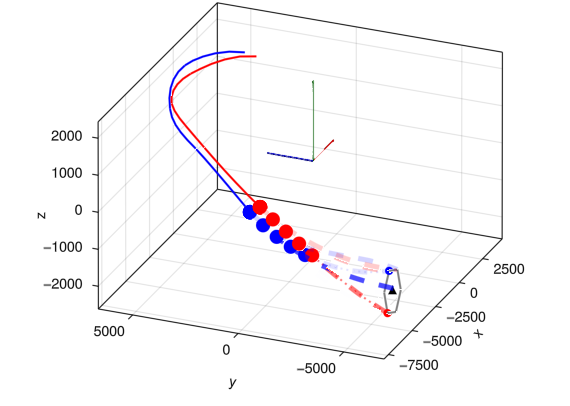
\includegraphics[width=\linewidth]{images/k_replan_5.png}
        \caption{Game step $s = 5$ }
        \label{fig:k_replan_5}
    \end{subfigure}
    \begin{subfigure}{0.32\linewidth}
        \centering
        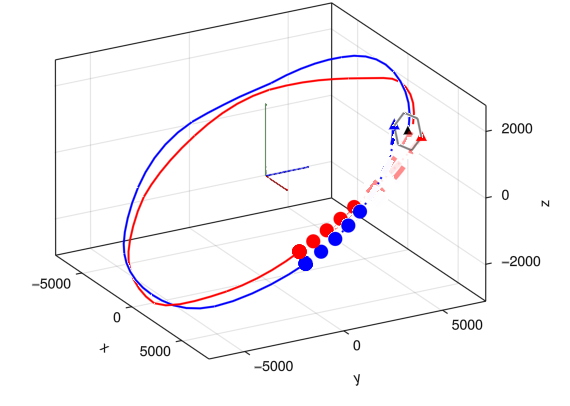
\includegraphics[width=\linewidth]{images/k_replan_10.png}
        \caption{Game step $s = 10$}
        \label{fig:k_replan_10}
    \end{subfigure}
    \caption{\textbf{Receding-horizon game, where blue shows the evader's path, and red represents the pursuer's.} The inertial frame's $x$, $y$, and $z$ axes are represented by the red, blue, and green arrows respectively. At each game step $s$, both players generate candidate trajectories, form the matrix game, and compute mixing weights. The solid lines represent the traveled trajectories in past game steps. For the current step, the thickness of the dashed lines represents each candidate trajectory's weight, and the spheres represent the chosen propagated states. }
    \label{fig:k_replan_all}
    \vspace{-1em}
\end{figure*}

% -------------

\subsection{Hexagonal Lifting}

The reference orbit is discretized into $K$ segments. At the evader's reference position one horizon ahead, $\bar{\mathbf{r}} = \bar{\mathbf{r}}_E(t_{k+L})$ with velocity $\bar{\mathbf{v}}$, we define the local directions
%
\begin{equation}
\hat{\mathbf{e}}_1 = \frac{\bar{\mathbf{v}}}{\|\bar{\mathbf{v}}\|}, \quad
\hat{\mathbf{e}}_2 = -\frac{\bar{\mathbf{r}}}{\|\bar{\mathbf{r}}\|}, \quad
\hat{\mathbf{e}}_3 = \frac{\hat{\mathbf{e}}_1 \times \hat{\mathbf{e}}_2}{\|\hat{\mathbf{e}}_1 \times \hat{\mathbf{e}}_2\|},
\label{eq:frame}
\end{equation}
%
i.e., prograde, nadir, and orbit normal. On a non-circular orbit $\hat{\mathbf{e}}_1$ and $\hat{\mathbf{e}}_2$ are not exactly orthogonal ($\hat{\mathbf{e}}_1 \cdot \hat{\mathbf{e}}_2 = -\sin\gamma$, with $\gamma$ the flight-path angle, $|\gamma| \lesssim e$), but $\hat{\mathbf{e}}_2$ and $\hat{\mathbf{e}}_3$ are orthonormal. A regular hexagon of radius $R$ is centered at $\bar{\mathbf{r}}$ in the nadir--normal ($\hat{\mathbf{e}}_2$--$\hat{\mathbf{e}}_3$) plane, with vertices
%
\begin{equation}
\mathbf{r}_{v_j} = \bar{\mathbf{r}} + R\left(\cos\theta_j\, \hat{\mathbf{e}}_3 + \sin\theta_j\, \hat{\mathbf{e}}_2\right), \quad \theta_j = \tfrac{\pi}{3}(j-1),
\label{eq:vertices}
\end{equation}
%
for $j = 1, \dots, 6$. Both players target the same six vertices. The vertices are a finite sample of the positions the evader may occupy one horizon ahead. \red{[TODO: forward reference to the lifting-bound section, which bounds the error of this restriction.]}

% -------------

\subsection{Candidate Trajectory Generation}

For each vertex $v_j$, player $i$ computes an $L$-impulse trajectory $\mathbf{U}_i^{(j)}$ that reaches it with minimum fuel by solving
%
\begin{equation}
    \begin{aligned}
        \min_{\mathbf{U}_i} \quad & \sum_{k=0}^{L-1} \sqrt{\|\mathbf{u}_i(t_k)\|_2^2 + \delta^2} \; + \; w\,\big\|\mathbf{r}_i(t_L) - \mathbf{r}_{v_j}\big\|_2 \\
        \text{subject to} \quad & \eqref{eq:state_eom}, \quad \|\mathbf{u}_i(t_k)\|_2 \leq \Delta V_{\max} .
    \end{aligned}
    \label{eq:mpc}
\end{equation}
%
The first term is the total $\Delta V$, smoothed by $\delta = 10^{-12}$ km/s so its gradient exists at zero impulse. The second is an exact penalty ($w = 1$) on the terminal \emph{position} miss. Problem \eqref{eq:mpc} is a nonconvex nonlinear program in $3L$ variables, and we solve it to local optimality. A Lambert solution provides the initial guess \cite{vallado2001fundamentals}. Gradients are computed by forward-mode automatic differentiation through the Kepler propagation, and the problem is solved with L-BFGS and a backtracking line search. Because the impulse bound never binds in our scenario (by more than an order of magnitude), we solve without it and verify it afterward; an augmented-Lagrangian loop enforces it if it is ever violated. Infeasible trial steps that make the propagation diverge are assigned a large finite cost, so the line search backs off.

% -------------

\subsection{The Matrix Game}

Let $j$ index the evader's candidate and $l$ the pursuer's. For every pair, the payoff is the horizon-averaged stage payoff \eqref{eq:objective} along the two candidate trajectories:
%
\begin{equation}
    A_{jl} = J\big(\mathbf{U}_E^{(j)}, \mathbf{U}_P^{(l)}\big) = \frac{1}{L} \sum_{k=0}^{L-1} \sqrt{d_k^{(j,l)} + \epsilon},
    \label{eq:ave_stage_cost}
\end{equation}
%
where $d_k^{(j,l)}$ is the separation \eqref{eq:distance} at $t_k$ when the evader flies candidate $j$ and the pursuer flies candidate $l$. This gives a $6 \times 6$ payoff matrix $\mathbf{A}$ in which the evader is the row player and \emph{maximizes} $A_{jl}$, and the pursuer is the column player and \emph{minimizes} it.

% ------------

\subsection{Mixed Strategies via Linear Programming}

A mixed strategy is a probability vector over the six candidates: $\mathbf{p} \in \Delta^6$ for the evader and $\mathbf{q} \in \Delta^6$ for the pursuer, where $\Delta^6 = \{\mathbf{w} \in \mathbb{R}^6 : \mathbf{w} \geq 0, \mathbf{1}^\top \mathbf{w} = 1\}$. The evader's security strategy maximizes its guaranteed payoff, and the pursuer's minimizes the payoff it can be forced to concede:
%
\begin{equation}
    \mathbf{p}^* \in \arg\max_{\mathbf{p} \in \Delta^6} \min_{l} \big(\mathbf{A}^\top \mathbf{p}\big)_l, \qquad
    \mathbf{q}^* \in \arg\min_{\mathbf{q} \in \Delta^6} \max_{j} \big(\mathbf{A} \mathbf{q}\big)_j .
    \label{eq:security}
\end{equation}
%
Each is computed by a linear program \cite{bacsar1998dynamic}. Shift the matrix so all entries are at least one, with $c_E = 1 + \max_{jl} A_{jl}$ and $c_P = 1 - \min_{jl} A_{jl}$. The evader solves
%
\begin{equation}
    \max_{\mathbf{z} \geq 0} \; \mathbf{1}^\top \mathbf{z} \quad \text{s.t.} \quad \big(c_E \mathbf{1}\mathbf{1}^\top - \mathbf{A}\big)^\top \mathbf{z} \leq \mathbf{1},
    \label{eq:game_LP}
\end{equation}
%
and the pursuer solves
%
\begin{equation}
    \max_{\mathbf{y} \geq 0} \; \mathbf{1}^\top \mathbf{y} \quad \text{s.t.} \quad \big(\mathbf{A} + c_P \mathbf{1}\mathbf{1}^\top\big)\, \mathbf{y} \leq \mathbf{1} .
    \label{eq:game_LP_P}
\end{equation}
%
Normalizing gives the mixing weights $\mathbf{p}^* = \mathbf{z}^*/\mathbf{1}^\top\mathbf{z}^*$ and $\mathbf{q}^* = \mathbf{y}^*/\mathbf{1}^\top\mathbf{y}^*$, and the two programs return the lower and upper values $c_E - 1/\mathbf{1}^\top\mathbf{z}^*$ and $1/\mathbf{1}^\top\mathbf{y}^* - c_P$. By the minimax theorem these coincide, and we call their common value $V$ the \emph{game value}. We reserve that term for $V$; realized outcomes are reported as mean separation. Each solution is checked against the saddle-point conditions,
%
\begin{equation}
    \max_j \big(\mathbf{A}\mathbf{q}^*\big)_j \;\leq\; V \;\leq\; \min_l \big(\mathbf{A}^\top \mathbf{p}^*\big)_l ,
    \label{eq:certificate}
\end{equation}
%
together with $\mathbf{p}^{*\top}\mathbf{A}\mathbf{q}^* = V$ and simplex feasibility, all to a relative tolerance of $10^{-8}$. A pair satisfying \eqref{eq:certificate} is a Nash equilibrium of the matrix game regardless of which solver produced it.

% --------------

\subsection{Receding-Horizon Fictitious Play}

Three time scales nest:
%
\begin{enumerate}
    \item Segment $k \in \{1, \dots, K\}$: the temporal discretization of the orbit.
    \item Horizon $L$: the number of segments in each candidate trajectory.
    \item Game step $s \in \{1, \dots, S\}$: the decision interval, spanning $N < L$ segments.
\end{enumerate}
%
At each game step, starting at $t_k$, each player generates its candidates over $[t_k, t_{k+L}]$, the matrix game is formed and solved, and each player selects a candidate according to its strategy (Section~\ref{sec:strategies}). Both players execute the first $N$ segments of their chosen trajectories, the clock advances to $t_{k+N}$, and the process repeats.

\subsubsection{Empirical Belief Update}

This update is used only by the fictitious-play (FP) strategies. After step $s-1$, each player observes the vertex its opponent chose. Let $\mathbf{g}_P \in \{0,1\}^6$ be the one-hot vector of the pursuer's choice and $\mathbf{g}_E$ that of the evader's. The evader keeps counts $\mathbf{f}_E \in \mathbb{R}^6$ of the pursuer's past choices and the pursuer keeps counts $\mathbf{f}_P$ of the evader's, both initialized to $\mathbf{1}$ (a uniform prior):
%
\begin{equation}
    \mathbf{f}_{E,s} = \mathbf{f}_{E,s-1} + \mathbf{g}_{P,s-1}, \qquad
    \mathbf{f}_{P,s} = \mathbf{f}_{P,s-1} + \mathbf{g}_{E,s-1} .
\end{equation}
%
Normalizing gives each player's belief about its opponent's mixed strategy: the evader's estimate of $\mathbf{q}$ and the pursuer's estimate of $\mathbf{p}$,
%
\begin{equation}
    \hat{\mathbf{q}}_s = \frac{\mathbf{f}_{E,s}}{\mathbf{1}^\top \mathbf{f}_{E,s}}, \qquad
    \hat{\mathbf{p}}_s = \frac{\mathbf{f}_{P,s}}{\mathbf{1}^\top \mathbf{f}_{P,s}} .
    \label{eq:belief}
\end{equation}
%
The belief pools observations from all past game steps, each of which has a different payoff matrix. It is meaningful because vertex $j$ denotes the same direction in the local frame \eqref{eq:frame} at every step, so the belief describes the opponent's \emph{decision rule} rather than any one game.

\subsubsection{Expected Payoff Under the Belief}

Under its belief, each player's expected payoff for each of its own candidates is
%
\begin{equation}
    \mathbf{c}_E = \mathbf{A}\,\hat{\mathbf{q}}, \qquad
    \mathbf{c}_P = -\mathbf{A}^\top \hat{\mathbf{p}},
    \label{eq:best_response}
\end{equation}
%
where the transpose reflects the pursuer's column role and the negation makes larger entries better for the pursuer, so both players maximize their own $\mathbf{c}$.

% --------------

\subsection{Strategies}
\label{sec:strategies}

Writing $\mathbf{w}^*$ for a player's own equilibrium weights ($\mathbf{p}^*$ or $\mathbf{q}^*$) and $\mathbf{c}$ for its expected payoff \eqref{eq:best_response}, each player uses one of five strategies:
%
\begin{enumerate}
    \item \textbf{Mixed}: sample a candidate from $\mathbf{w}^*$. This is the security strategy: in expectation it guarantees $V$ in the stage game against any opponent.
    \item \textbf{Greedy}: select $\arg\max_j w^*_j$, the most heavily weighted candidate. This is a heuristic baseline: the equilibrium guarantee requires sampling the full distribution, so greedy forfeits it and is not a best response to anything.
    \item \textbf{Random}: select a candidate uniformly at random, independent of $\mathbf{A}$.
    \item \textbf{FP-greedy}: select $\arg\max_j c_j$, the best response to the belief \eqref{eq:belief}.
    \item \textbf{FP-mixed}: sample candidate $j$ with probability proportional to $c_j - \min_m c_m + 10^{-6}$. This heuristic stochastic variant of fictitious play favors better responses without committing to one; it is non-negative and unchanged by adding a constant to $\mathbf{c}$, and it gives the worst candidate almost zero probability.
\end{enumerate}
